\ProvidesFile{ch-light-curve-simulation.tex}[Light Curve Simulation]
\graphicspath{{/Users/liamrobinson/Documents/PyLightCurves/docs/build/html/_images}}

\section{Light Curve Simulation}

\subsection{Orbit Propagation}

There are many environmental perturbations that effect the natural motion of space objects in orbits around Earth. In LEO, drag and the $J_2$ term of Earth's gravity field due to equatorial oblateness are the dominant perturbations \cite{frueh2019notes}. In MEO and GEO, solar radiation pressure (SRP) and the third-body effects of the Sun and Moon become increasingly important while drag is negligible \cite{frueh2019notes}. For the purposes of accurate light curve simulation, the orbit propagation must be accurate enough for the hour to week-long scenarios, and it should also be easy to access real initial conditions for objects of interest near the propagation dates. The Simplified General Perturbations 4 (SGP4) propagator fits these needs well. SGP4 models the secular effects of the first few zonal terms of Earth's gravity field, drag through an exponential density atmosphere, and some of the effects of third bodies like the Sun and Moon \cite{vallado4ed}. The propagator takes as input a Two-Line Element (TLE) set along with the Julian dates to propagate the object to and returns the position and velocity in TEME \cite{vallado4ed}. TLEs themselves are short, standardized collections of orbital elements and mission information, produced from recent observations of the object in question. TLEs are available programatically through Space-Track, a service provided by the US Space Force's 18th Space Defense Squadron \cite{spacetrack}. While SGP4 does not model some important perturbations like SRP, the availability of frequently updated TLEs for regularly tracked objects alleviates most concerns, although errors on the order of a few kilometers are still expected for LEO objects \cite{vallado4ed}. 

Orbital propagation for the simulations performed in this work was done using SGP4 with TLE interpolation. For a given set of Julian dates and the satellite name in question, Space-Track is queried to find all TLEs produced for that object in the interval of interest. SGP4 is run for all Julian dates and all TLEs, and the final position at each Julian Date is simply linearly interpolates between the most recent past TLE and the next future TLE. If there is only one neighboring TLE, its position is used without interpolation.

\subsection{Discrete Shape Representations}

A computer can represent 3D objects implicitly or explicitly. An implicit representation might be the solution to an algebraic equation, i.e., $x^2 + y^2 + z^2 = 1$ defines a sphere of radius $1$ centered at the origin. Often, a shape may be defined by a set of signed distance functions (SDFs). An SDF takes in a point in \rthree and outputs the distance from the object, returning negative distance if the queried point is inside the shape. The object can then be rendered via ray marching. A ray is cast from the camera out into the scene for each pixel of the screen, each performing distance queries along its length until it intersects the object or diverges. 

By contrast, an explicit shape representation creates complex 3D geometry from simple 2D building blocks. In the most common case, object faces are defined by triangles. This means that at the scale of the individual faces, the shape is always composed of flat surfaces that meet at sharp angles. While this can add complexity to many fields of shape analysis and geometry processing, triangulated surfaces are perfect for light curve shape inversion. Human-made space objects like most satellites are composed of flat faces, with the exception of parabolic antennas and cylindrical rocket bodies.

\subsubsection{The Object File Format}

One common text file format for 3D model files is \texttt{.obj}, developed by Wavefront Technologies in the early 1990s \cite{obj_format}. Each OBJ file consists of a list of vertex positions and face definitions, with optional vertex normals and tangents. An \texttt{.obj} listing for a cube is included for reference in Appendix \ref{sec:obj_listing}. Given the vertex positions and adjacency information stored in the model file, useful properties of the object can be computed for use later in both light curve simulation and shape inversion. 

\subsubsection{Properties of Triangulated Meshes}

For each triangular face $F_i$ of the model defined by vertices $F_i = \left\{v_1, v_2, v_3\right\}$, the outward-pointing face normal is computed with:

\begin{equation} \label{eq:face_normal}
    \hat{n} = \frac{\left( v_2 - v_1 \right) \times \left( v_3 - v_1 \right)}{\| \left( v_2 - v_1 \right) \times \left( v_3 - v_1 \right) \|_2}.
\end{equation}

The face area is computed with:

\begin{equation} \label{eq:face_areas}
    a = \frac{\| \left( v_2 - v_1 \right) \times \left( v_3 - v_1 \right)\|_2}{2}.
\end{equation}

The support of the $i$th face --- the perpendicular distance from the origin to the plane defining the face --- is computed with the position of any vertex on that face, i.e., the first vertex $v_{i,1}$, and the face normal vector $\hat{n}_i$:

\begin{equation} \label{eq:face_support}
    h_i = v_{i,1} \cdot \hat{n}_i.
\end{equation}

The volume of the object is computed:

\begin{equation} \label{eq:object_volume}
    V = \frac{1}{3} \sum_{i=0}^{ \lvert F \rvert}\vec{h}_i \cdot \vec{a}_i.
\end{equation}

In Eq \ref{eq:object_volume}, $\lvert F \rvert$ is the number of faces defining the object. $\vec{h}$ and $\vec{a}$ are column vectors collecting all face supports and areas. The Extended Gaussian Image, a quantity defined in \ref{sec:egi_definition}, is computed row-wise for the $i$th face with:

\begin{equation} \label{eq:egi_definition}
    \vec{E}_i = \vec{a}_i \vec{n}_i.
\end{equation}

\subsection{Selected Satellite Models}

Most of the analysis in this work used one of the 3D model files shown in Figure \ref{fig:satellite_lineup}. Figure \ref{fig:satellite_lineup} highlights the size of the GEO communications satellites (TELSTAR, HYLAS, Hispasat, and ASTRA). In contrast, the LEO satellites (Starlink and Landsat) are dwarfed at the left end of the lineup.

\begin{figure}[ht]
    \centering
    \includegraphics[width=\figbig]{sphx_glr_satellite_lineup_001.png}
    \caption{Selected space objects with soccer field for size reference. In order, the objects are TESS, Starlink V1, TDRS, Landsat 8, Hispasat 30W-6, Saturn V SII, TELSTAR 19V, HYLAS 4, and simplified ASTRA.
    }
    \label{fig:satellite_lineup}
\end{figure}

\subsection{The Bidirectional Reflectance Distribution Function}

Although light curves come from unresolved measurements, the interactions that produce them are directly driven by the shape and material properties of the object being observed. In order to simulate accurate light curves, all relevant optical interactions must be modeled. In broad terms, this boils down to determining how the object is illuminated, how it casts shadows on itself, and how it is observed. 

At the microscopic scale, the surface of an object is composed of facets ---  small areas sharing a normal vector. The macroscopic optical properties of the material is driven by the distribution of sizes and normal directions of these microfacets. If the facet normals are distributed in biased orientations, the macroscopic surface may show anisotropy, leading to the appearance of brushed metal. If the facets normals are at large angles to each other, the surface may appear dull as the direction of the outgoing light may be largely independent from the incoming direction. Subsurface effects ---  where incoming light rays scatter \textit{inside} the surface can also change the macroscopic properties of the material. 

This discussion raises an important question; how should the macroscopic outcomes of the microscopic interactions of incident light on a surface be modeled? The bidirectional reflectance distribution function (BRDF) is a tool from computer graphics that addresses this problem. The BRDF is a function on the hemisphere which expresses the fraction of light per solid angle (radiance $\mathcal{R}$) leaving the surface in a given direction, divided by the incident power per unit area (irradiance $\mathcal{I}$). The general formulation for a BRDF $f_r$ is given by \cite{duvenhage2013}:

\begin{equation} \label{eq:brdf_def}
    f_r(\vctr{x}, L \rightarrow O) = \frac{d\mathcal{R}\left(\vctr{x} \rightarrow O\right)}{d\mathcal{I}\left(L \rightarrow \vctr{x}\right)}.
\end{equation}

In Eq \ref{eq:brdf_def}, $\vctr{x} \in \mathbb{R}^3$ is the point on the object's surface where the BRDF is evaluated. $L \in \mathbb{S}^2$ is the incoming illumination unit vector and $O \in \mathbb{S}^2$ is the outgoing unit vector. Note that this work treats $f_r(\vctr{x}, L \rightarrow O)$ and $f_r(L \rightarrow O)$ as equivalent in later descriptions, leaving the evaluation point $\vctr{x}$ implied. This definition is useful for building intuition about the form of the BRDF, but to represent a physically plausible reflection process, a candidate function must satisfy three additional constraints. A physically plausible BRDF must conserve energy --- more energy cannot be reflected from the surface than was incident on it. It must also be reciprocal --- switching the observer and illumination directions should not change the BRDF value as the surface interaction. This reciprocity is sometimes known as the \textit{Helmholtz Reciprocity Rule} in literature \cite{montes2012}. Finally, plausible BRDFs are positive --- they take on nonnegative values for all valid inputs \cite{montes2012}. A surface cannot reflect negative light, so this should feel natural. Explicitly, energy conservation is expressed with \cite{montes2012}:

\begin{equation} \label{eq:brdf_energy_cons}
  \forall L \in \mathbb{S}^2 : \:\: \int_{O \in \mathbb{S}^2} f_r(L \rightarrow O) \: d\mathbb{S}^2 \leq 1.
\end{equation}

Eq \ref{eq:brdf_energy_cons} states that for all possible illumination directions $L$, integrating all possible outgoing observer directions $O$ on the unit sphere cannot return greater than one from the energy conservation integral. Reciprocity can be formalized as:

\begin{equation} \label{eq:brdf_reciprocity}
  \forall L, O \in \mathbb{S}^2 : \:\: f_r(L \rightarrow O) = f_r(O \rightarrow L).
\end{equation}

\subsection{BRDF Formulations}

Now that the requirements for a plausible physical BRDF have been established, a collection of commonly-used BRDFs can be presented. The following BRDFs are all energy conserving, reciprocal, and nonnegative. This does not mean that they are always sufficient for modeling real-world materials, they merely represent ways hypothetical surfaces could reflect light without breaking any fundamental physics.

\subsubsection{Lambertian}

The simplest BRDF is one that reflects equally in all directions. This BRDF is termed Lambertian or diffuse.

\begin{equation} \label{eq:brdf_lambertian}
  f_r(L \rightarrow O) = \frac{C_d}{\pi}
\end{equation}

In Eq \ref{eq:brdf_lambertian}, $0 \leq C_d \leq 1$ is the surface's coefficient of diffuse reflection. For example, $C_d = 0.4$ means that the surface reflects $40\%$ of incident radiation and absorbs the other $60\%$. 

\subsubsection{Phong}

While the diffuse BRDF reflects energy isotropically, many real-world reflections are highly biased. At the extreme end, a perfect mirror reflection is effectively a Dirac delta function in the reflected illumination direction. Many real-world materials are well-modeled as a linear combination of diffuse and specular effects. A simple specular BRDF model is that developed by Phong in 1975 \cite{phong1975}. The Phong model splits the BRDF into a Lambertian term governed by $C_d$ and a specular term governed the coefficient of specular reflection $ 0 \leq C_s \leq 1$ and the specular exponent $n \geq 0$ \cite{duvenhage2013}. 

\begin{equation} \label{eq:brdf_phong}
  f_r(L \rightarrow O) = \frac{C_d}{\pi} + \frac{C_s \frac{n+2}{2\pi} (O \cdot R)^n}{N \cdot L}
\end{equation}

In Eq \ref{eq:brdf_phong}, $R$ is the reflected illumination vector, computed via $R = 2 (N \cdot L) N - L$. As $n$ increases, the specular glint becomes sharper and more intense, eventually approaching a perfectly mirror reflection. Because of the introduction of a new coefficient of reflection, a new constraint is needed to maintain energy conservation. Because $C_d$ and $C_s$ each represent the \textit{fraction} of light reflected in each mode, it should be clear that $C_d + C_s \leq 1$. This can also be reformulated with an explicit coefficient of absorption $C_a$ which captures the fraction of incident radiation absorbed by the surface, yielding $C_d + C_s + C_a = 1$. 

\subsubsection{Blinn-Phong}

The Blinn-Phong BRDF is similar to to the Phong BRDF, but parameterizes the specular lobe in terms of the halfway vector $H$ \cite{duvenhage2013}. This vector is halfway between the illumination and observer directions such that $H = L + O$ which needs to be normalized before use. As the halfway vector approaches the surface normal vector, the observer must be approaching the reflected illumination vector, leading to a more intense specular highlight. 

\begin{equation} \label{eq:brdf_blinn_phong}
  f_r(L \rightarrow O) = \frac{C_d}{\pi} + \frac{C_s \frac{n+2}{2\pi} (N \cdot H)^n}{4 (N \cdot L)(N \cdot O)}
\end{equation}

\subsubsection{Glossy}

The so-called glossy BRDF simulates reflections from plastic materials using an Gaussian distribution around the specular scattering lobe \cite{duvenhage2013}:

\begin{equation} \label{eq:brdf_glossy}
  f_r(L \rightarrow O) = \frac{C_d}{\pi} + \frac{C_s}{2\pi \sigma^2 \left(N \cdot L\right)}  e^{\frac{-\left( R \cdot O \right)^2}{2\sigma^2}},
\end{equation}

where the parameter $\sigma$ controls the width of the specular Gaussian.

\subsubsection{Cook-Torrance}

The Cook-Torrance explicitly accounts for the orientation of the microfacets making up the surface \cite{cook1982}. This model is built from a facet slope distribution term $D$, a Fresnel term $F$, and a geometric attenuation factor $G$. The slope distribution term describes the probability density of a given facet being oriented with a normal vector aligned with the halfway vector $H$ \cite{cook1982}. A common formulation of this term is due to Beckmann:

\begin{equation} \label{eq:d_beckmann}
  D = \frac{1}{\pi \alpha^2 \left( N \cdot H \right)^4} \exp\left( \frac{1 - \left(N \cdot H\right)^2}{\alpha^2 \left(N \cdot H\right)^2} \right).
\end{equation}

In Eq \ref{eq:d_beckmann}, $\alpha \in [0, 1]$ is the roughness of the surface \cite{cook1982}. The Fresnel term accounts for the variation in specular reflection due to the angle of incidence. In reality, this term is a function of wavelength, but is often approximated as \cite{cook1982}:

\begin{equation} \label{eq:fresnel_approx}
  F = C_s + \left( 1 - C_s \right) \left( 1 - \left( H \cdot L \right) \right) ^ 5.
\end{equation}

The geometric attenuation term expresses how microfacets shadow eachother, and can be approximated with \cite{cook1982}:

\begin{equation} \label{eq:cook_torrance_g}
  G = \min \left\{ 1, \frac{2\left(N \cdot H\right) \left(N \cdot O\right)}{O \cdot H}, \frac{2\left(N \cdot H\right) \left(N \cdot L\right)}{O \cdot H} \right\}.
\end{equation}

The overall reflectance for the Cook-Torrance BRDF is given by:

\begin{equation} \label{eq:brdf_cook_torrance}
  f_r(L \rightarrow O) = \frac{C_d}{\pi} + \frac{D \cdot G \cdot F}{4 \left(N \cdot L\right) \left( N \cdot O \right)}
\end{equation}

\subsubsection{Oren-Nayar}

The Oren-Nayar BRDF is an improved model of diffuse reflectance for many real-world materials like ceramics and the surface of the Moon. These materials diverge from the Lambertian model near the horizon, reflecting much more light than would be predicted by simple cosine loss \cite{oren1994}. This BRDF relies on the surface roughness $\alpha$ to compute a set of constants \cite{oren1994}:

\begin{align*} \numberthis
  A &= 1 - 0.5 * \frac{\alpha^2}{\alpha^2 + 0.33} \\
  B &= 0.45 * \frac{\alpha^2}{\alpha^2 + 0.09} \\
  C &= \frac{\mathrm{proj}_{N}\left(L\right)}{\|\mathrm{proj}_{N}\left(L\right)\|} \cdot  \frac{\mathrm{proj}_{N}\left(O\right)}{\|\mathrm{proj}_{N}\left(O\right)\|}. \\
  \beta &= \max \left\{ \arccos\left( L \cdot N \right), \: \arccos\left( O \cdot N \right) \right\} \\
  \gamma &= \min \left\{ \arccos\left( L \cdot N \right), \: \arccos\left( O \cdot N \right) \right\} \\
\end{align*}

With these values computed, the reflectance of the Oren-Nayar BRDF is given by \cite{oren1994}:

\begin{equation}
  f_r(L \rightarrow O) = \frac{C_d}{\pi} \left(A + (B \max\left\{C, 0\right\} \sin\beta \tan\gamma) \right)
\end{equation}

\subsubsection{Ashikhmin-Shirley}

The Ashikhmin-Shirley BRDF is unique among those presented in this section as it allows for anisotropic reflection which can be non-negligible for metals \cite{ashikhmin2000}. This model is parameterized by the diffuse reflection coefficient, as well as two specular exponents $n_u$ and $n_v$. When $n_u = n_v$, the model behaves much like the Phong BRDF. The full BRDF is expressed \cite{ashikhmin2000}:

\begin{align*} \numberthis \label{eq:brdf_ashikhmin_shirley}
  \rho_d &= \frac{28 C_d}{23 \pi} (1 - C_s) \left(1 - \left(1 - \frac{N \cdot L}{2}\right)^5\right) \left(1 - \left(1 - \frac{N \cdot O}{2}\right)^5\right) \\
  \rho_s &= \frac{\sqrt{(n_u+1)(n_v+1)}}{8 \pi} \frac{\left( N \cdot H \right)
  ^\frac{n_u \left(H \cdot U \right)^2 + n_v \left( H \cdot V \right)^2}{1 - \left(H \cdot N\right)^2}}
  {\left(H \cdot L\right) \max\left\{ N \cdot O, N \cdot L \right\}} F \\
  f_r(L \rightarrow O) &= \rho_d + \rho_s. \\
\end{align*}

In Eq \ref{eq:brdf_ashikhmin_shirley}, $F$ is the same Fresnel factor in Eq \ref{eq:fresnel_approx} while $U$ and $V$ are predefined surface basis vectors perpendicular to the surface normal.

\subsection{BRDF Summary}

\begin{figure}[ht]
  \centering
  \includegraphics[width=\figbig]{sphx_glr_brdf_renders_002_2_00x.png}
  \caption{Implemented BRDFs rendered with arbitrary parameters, demonstrating the qualitative differences between lighting models}
  \label{fig:brdf_renders}
\end{figure} 

\subsection{Real Material Properties}

Producing accurate light curves requires accurate optical properties for the simulated materials. Matusik et al. compiled measured bidirectional reflectance data from over 100 real materials including various metals and paints that might be found on human-made space objects \cite{matusik2003}. Optimally, such a dataset would be used to model the structure, solar panels, and antenna surfaces of the simulated objects. However, it is far more computationally efficient to fit one of the presented three parameter BRDFs to observed data. The Phong model parameters used for simulations in this work are listed in Table \ref{tb:real_matprops}.

\begin{table}[]
  \centering
  \begin{tabular}{|l|l|l|l|}
  \hline
  \textbf{Material} & $C_d$ & $C_s$ & $n$ \\ \hline
  Solar panel (Phong) \cite{fankhauser2023}              & $0.15$ & $0.25$ & $0.26$  \\ \hline
  Bus structure (Phong) \cite{fankhauser2023}               & $0.34$ & $0.40$ & $8.9$  \\ \hline
  Multilayer insulation (MLI) (Phong) & $0.1$ & $0.9$ & $20$ \\ \hline
  White paint (Phong) & $0.9$ & $0.1$ & $1$ \\ \hline
  \end{tabular}
  \caption{Reflection properties of real materials. MLI and white paint parameters are estimated. Significant variance may exist depending on surface finishes.}
  \label{tb:real_matprops}
\end{table}

\subsection{Simulating Normalized Light Curves of Convex Objects}

Light curve simulation for convex geometry can be solved semi-analytically as each face's contribution 
to the measured irradiance can be computed individually \cite{kaasalainen2001}. 
Determining whether a face is illuminated requires two horizon checks to determine visibility 
from the Sun and to the observer. For a face $i$ at timestep $j$ these horizon checks are 
expressed by the shadowing condition $\mu_{ij}$. 

\begin{equation} \label{eq:cvx_shadow_cond}
  \mu_{ij} = \begin{cases}
    1 \text{ if } \left( O_j \cdot \hat{n}_i \right) > 0 \text{ and } \left( L_j \cdot \hat{n}_i \right) > 0 
	  \text{ and } \delta_{ij,\text{ss}} = 0 \text{ and } \delta_{ij,\text{os}} = 0\\
    0 \text{ otherwise } \\
  \end{cases}
\end{equation}

The unit vectors $O$ and $L$ point from the center of mass of the object to the observer and Sun, respectively. The outward-pointing face normal unit vector $\hat{n}$ is chosen by convention for all mesh operations. 
The self-shadowing and observer-shadowing conditions, $\delta_{ij,\text{ss}}$ and $\delta_{ij,\text{os}}$, 
are always zero for convex polyhedra but are crucial for accurately simulating nonconvex geometry. 
For objects with concavities, self-shadowing refers to shadows cast by an object onto itself and observer-shadowing 
refers to otherwise visible faces blocked by other portions of the geometry.

The irradiance $I$ received by the observer at timestep $j$ is the sum of the received irradiance from all faces, where the BRDF is evaluated at each face. Each contribution is expressed as the product of the
normalized irradiance $\hat{I}$. This can be scaled to adjust for the distance from the observer to
the object and the solar constant to yield the noiseless received irradiance. For any physically plausible BRDF, the normalized light curve for a convex object is expressed as a sum over all faces $i$ at time step $j$:

\begin{equation} \label{eq:lc_func_normalized}
  \hat{I}_{j} = \sum_{i=1}^{m}{\mu_{ij} \mu_{Earth,j} a_i f_r(L_j \rightarrow O_j) \left( \hat{O}_j \cdot \hat{n}_i \right) \left( \hat{S}_j \cdot \hat{n}_i \right)}.
\end{equation}

In Eq \ref{eq:lc_func_normalized}, $a_i$ is the area of the $i$th face and $f_{Sun}$ is the solar irradiance fraction. Note that $f_r(L_j \rightarrow O_j)$ must be computed separately for each face to account for normal vector and coefficient of reflection differences. This normalized light curve can be dimensionalized by the total solar irradiance and the distance $r_j$ between the observer $\vctr{r}_{obs}$ to the object center of mass $\vctr{r}_{obj}$:

\begin{equation} \label{eq:lc_func_norm_to_irrad}
  I_{j} = \frac{I_0 \hat{I}_j}{r_j^2}.
\end{equation}

Note that using $r_j = \| \vctr{r}_{obj} - \vctr{r}_{obs} \|$ is a simplifying assumption as some faces of the object are further or closer to the Sun than the center of mass. As the scale of human-made space objects are a factor of $10^{10}$ to $10^{12}$ smaller than the distance to the Sun, the difference across the surface of the object is negligible.


\subsection{Simulating Normalized Light Curves of Nonconvex Objects}

Many existing light curve simulation methods for nonconvex objects rely on ray tracing schemes like Möller and Trumbore's ray-triangle intersection algorithm \cite{moller2005,fan2020thesis}. This computation has complexity $\mathcal{O}(n^2)$ if implemented naïvely, but can be improved to $\mathcal{O}(n \ln n)$ with better spatial data structures. For human-made space objects, there may be significant self-shadowing at large phase angles. As a result, it cannot be assumed that the self-shadowing conditions $\delta_{ij,\text{ss}}$ and $\delta_{ij,\text{os}}$ are zero \cite{frueh2014,fan2020thesis}. Naïve ray traced shadows generally require $\mathcal{O}(n^2)$ ray-triangle intersections per timestep for $n$ faces. For this reason, ray traced shadows quickly become infeasible for complex objects without GPU parallelization. The limitations of ray-triangle intersections for light curve simulation is discussed at length by Frueh et al. \cite{frueh2014}.

\graphicspath{{/Users/liamrobinson/Documents/msthesis/static_images/aas_2022_figs}}
\begin{figure}[!htb]
  \centering
  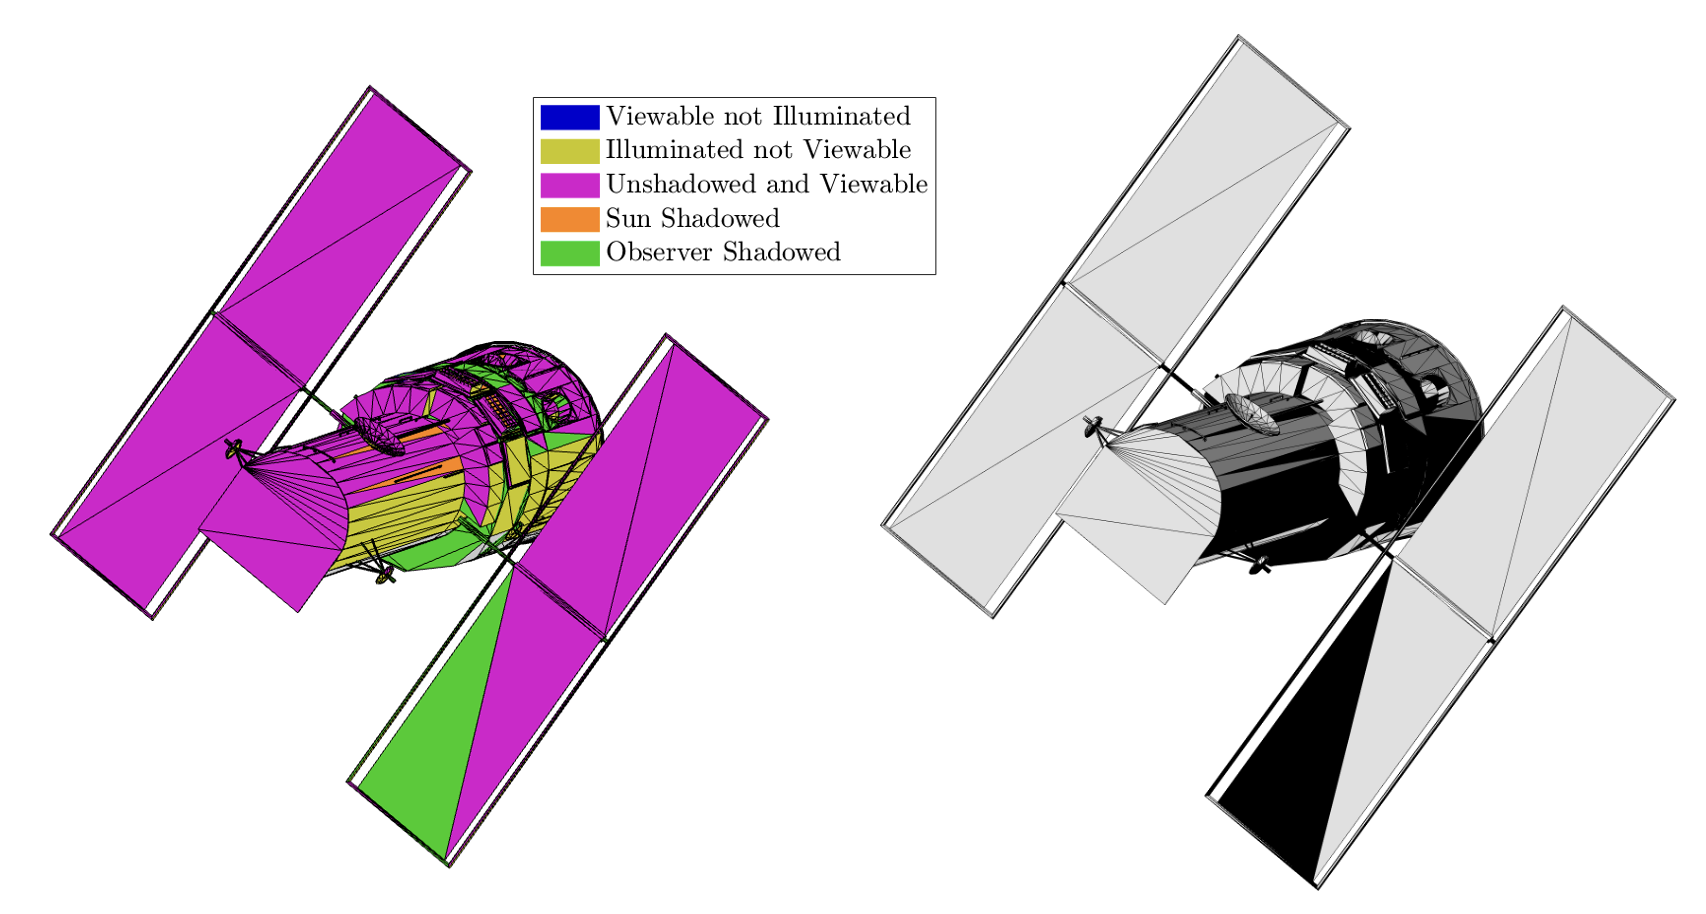
\includegraphics[width=350px]{hst_shadow_mapping/composite_hst_raytraced.png}
  \caption{Hubble Space Telescope ray traced shadow categorization and shading. Models from \cite{nasa_models}}
  \label{hst_shadows_ray}
\end{figure}

\subsubsection{The Importance of Self-Shadowing}

To motivate the need for accurate shadows when dealing with human-made space objects, consider the error introduced by neglecting shadows for different types of space objects. Kaasalainen and Torppa's work on asteroids reasonably assumed that shadowing was a negligible contribution to the measured light curve. Human-made objects do not afford the same luxury. Figure \ref{fig:hst_bennu_shadows} displays light curves for the asteroid Bennu and the Hubble Space Telescope with and without accurate shadows under a single-axis spin profile with inertially fixed Sun and observer vectors. Without accurate shadowing, the light curve's intensity and its time derivative can be significantly error-prone.

\begin{figure}[!htb]
  \centering
  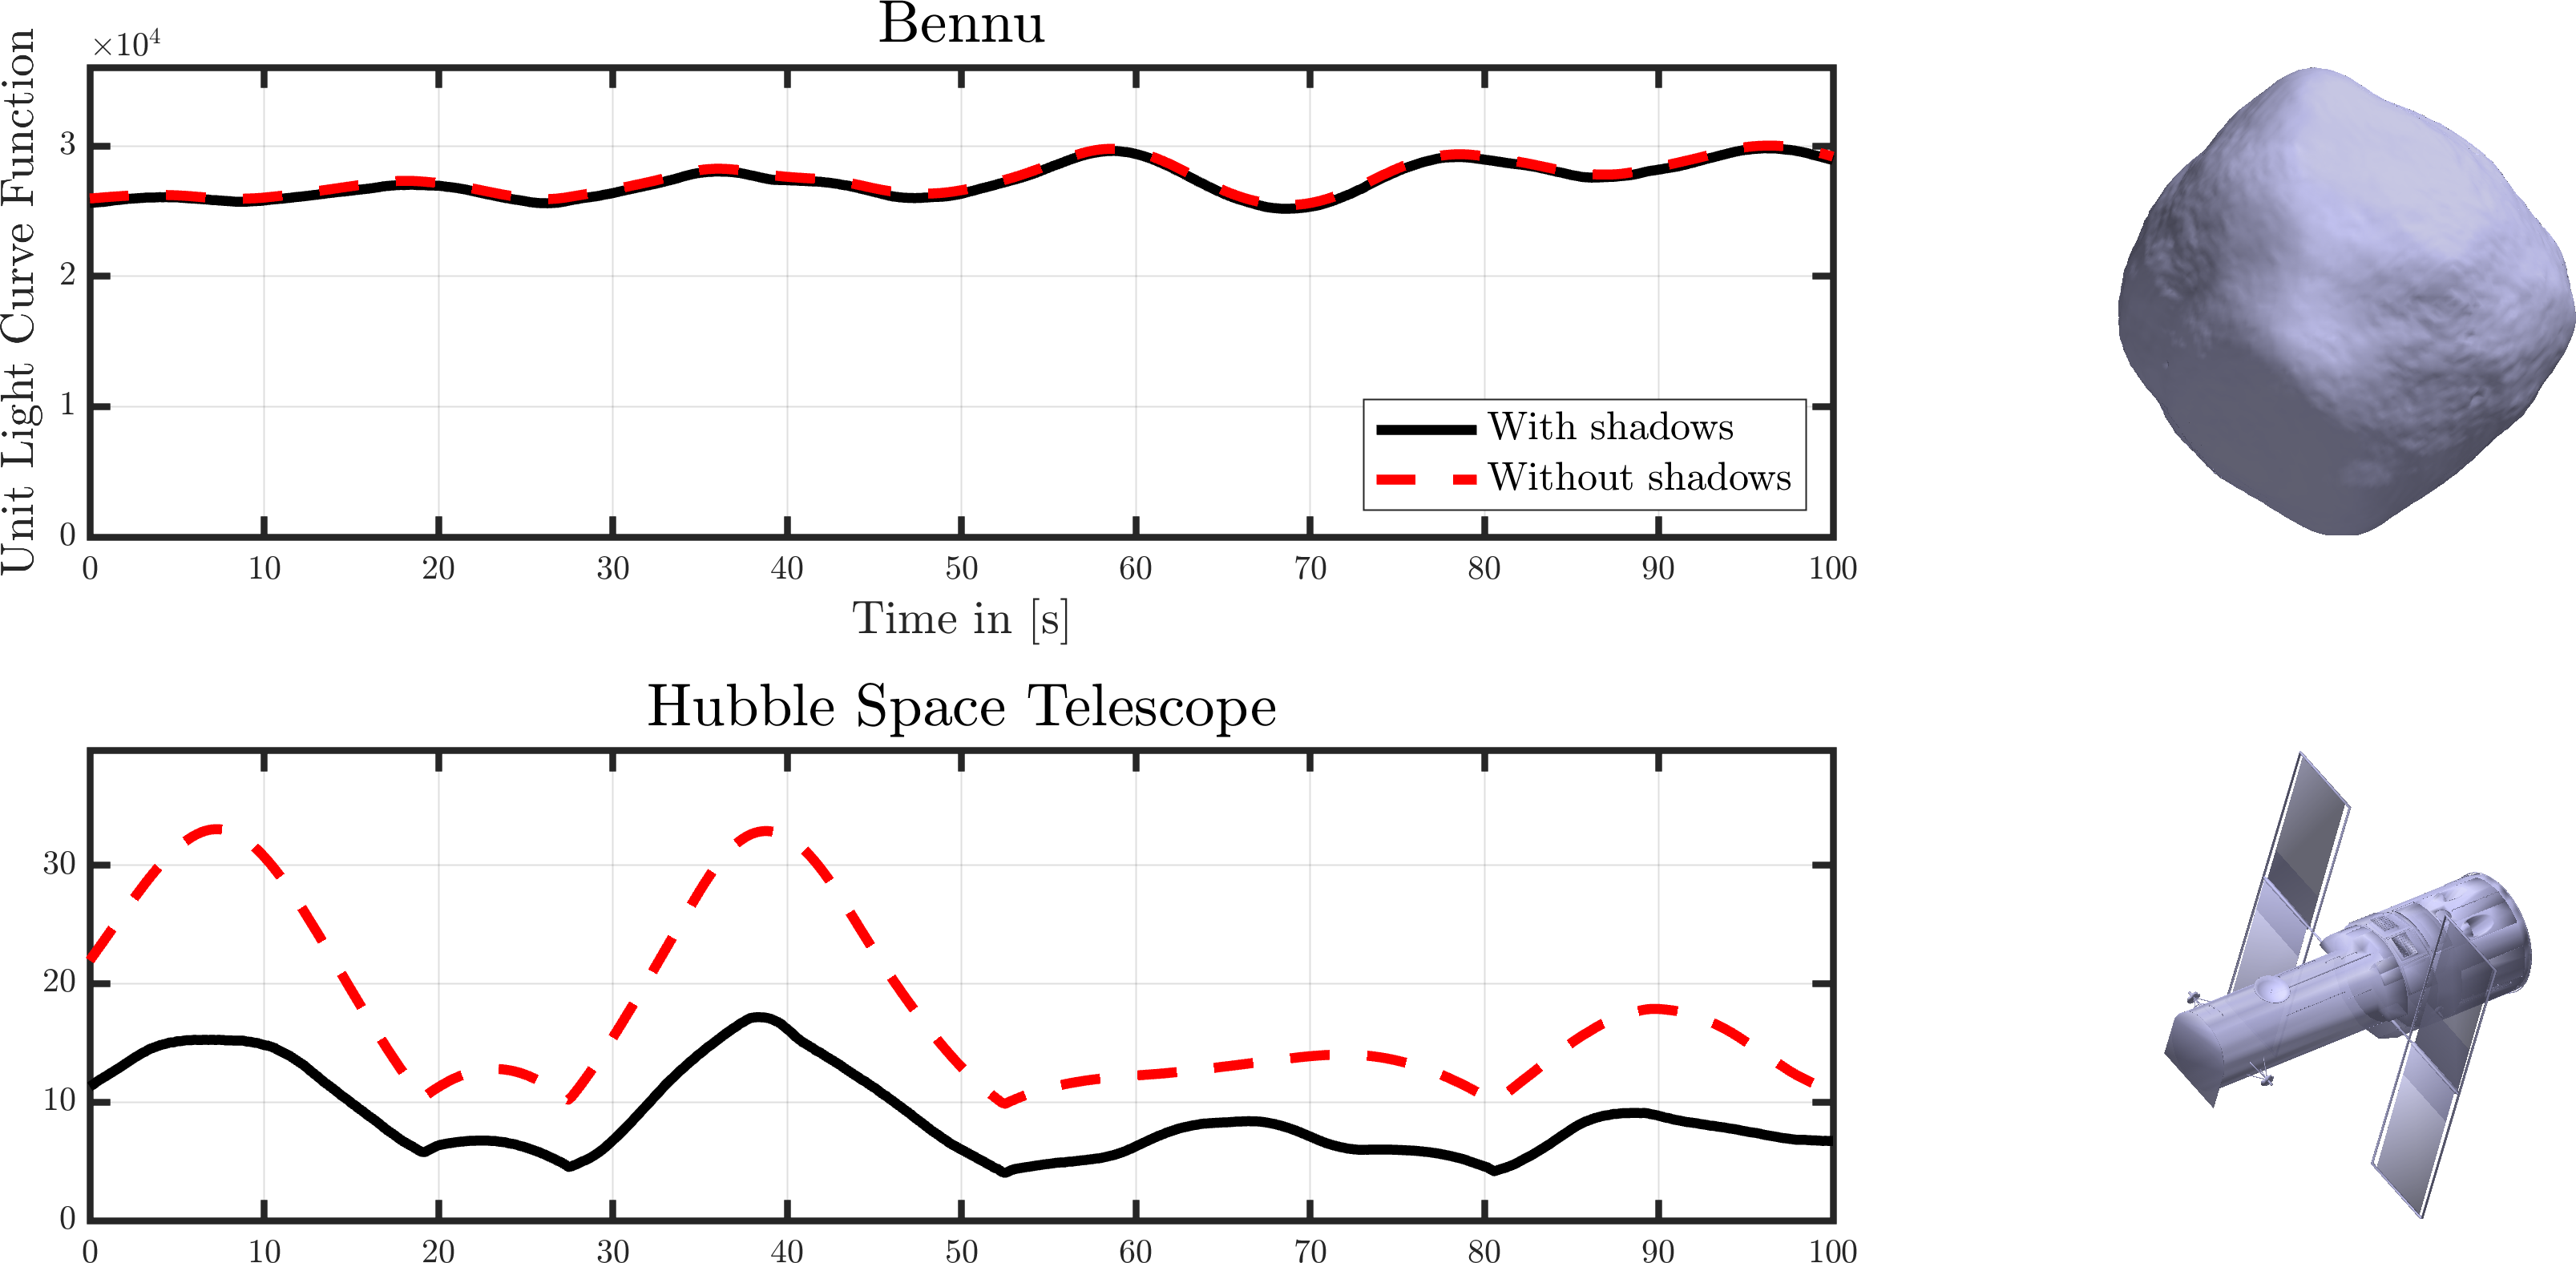
\includegraphics[width=350px]{convex_vs_nconv_lcs.png}
  \caption{Normalized irradiance errors introduced by neglecting shadows for Bennu and HST. Models from \cite{nasa_models}}
  \label{fig:hst_bennu_shadows}
\end{figure}

\subsubsection{Shadow Mapping} \label{sec:shadow_mapping}

Shadow mapping is used in the simulations presented in this work for faster and more accurate self-shadowing. Shadow mapping is a well understood technique in computer graphics \cite{kolivand2013}. Although modern ray traced shadowing may be more computationally efficient, shadow mapping was selected for its ease of implementation \cite{kolivand2013}. Shadow mapping shades individual pixel fragments instead of entire faces, offering increasing shadow quality over facewise ray tracing as the number of mesh faces falls.

Given an observer and Sun vector in the body frame of the object, shadow mapping proceeds in a four step process. In step one, a camera is positioned along the Sun vector and a perpendicular depth texture is computed. In the second step, depth values in Sun camera space are transformed to observer camera space, where a second depth texture is computed. This second texture is used to find the closest fragment along each ray to the Sun \cite{brabec2002}. Self-shadowed fragments are classified as those further from the Sun than the closest fragment along the same ray, indicated in red in Figure \ref{fig:hst_shadows_map}. Fragments that do not pass the convex shadowing condition are horizon shadowed, indicated in blue in Figure \ref{fig:hst_shadows_map}, determining the Sun and observer shadowing conditions at once. All remaining fragments are shaded with using the same Lambertian reflection model in \ref{eq:lc_func_normalized}. Computing the light curve function for the final rendered image requires summing all pixel values and dimensionalizing the result by the area of the observer camera's field of view. The light curve simulation environment used in this work was implemented in C and OpenGL \cite{raylib}.

In order to compute the final shaded and shadowed image, a depth map must be computed from the perspective of two orthographic cameras in the Sun and observer directions. These depth masks require a set of transformations from the model body frame to screen space. With this background laid out, the process for computing a perpendicular depth map $d(x,y)$ from the perspective of an arbitrary orthographic camera is detailed in Algorithm \ref{alg:depth_map}.

\begin{algorithm}
  \caption{Depth map for shadow mapping} \label{alg:depth_map}
  \begin{algorithmic}
    \State $(x, y) \in \mathbb{Z}$ \Comment{Pixel coordinates on the image plane}
    \State $R_{pix} \in \mathbb{R}^3$ \Comment{Pixel world coordinates; provided by OpenGL}
    \State $d(x, y) \gets \left( R_{cam} - R_{pix} \right) \cdot R_{cam}$ \Comment{Pixel depth in the camera view direction}
  \end{algorithmic}
\end{algorithm}

The pixel-wise shading process is summarized in Algorithm \ref{alg:pix_shading} in Appendix \ref{data:shading}. This shading and shadow mapping procedure is detailed graphically in Figure \ref{fig:hst_shadows_map}.

\begin{figure}[!htb]
  \centering
  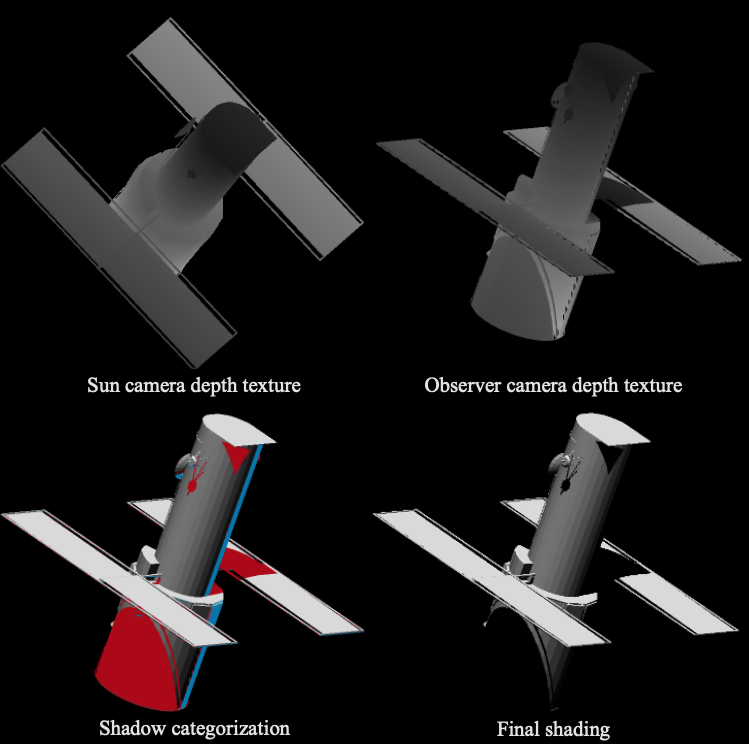
\includegraphics[width=\figmed]{hst_shadow_mapping/hst_shadow_mapping.png}
  \caption{Hubble Space Telescope shadow mapping with self (red) and horizon (blue) shadows rendered. Models from \cite{nasa_models}}
  \label{fig:hst_shadows_map}
\end{figure}

An image shaded by Algorithm \ref{alg:pix_shading} is dimensionalized to a normalized irradiance value by computing the area of the square orthographic field of view given the image pixel count $n_{pix}$:

\begin{equation} \label{eq:ortho_area}
  A_{image} = 2 n_{pix} \left(FOV \right)^2.
\end{equation}

This field of view must be set dynamically at runtime to account for the size of the 3D model. The pixel values $v$ in the image are stored as unsigned 8 bit integers which take on values from 0 to 255, corresponding to the power range 0 to 1 within the pixel shading procedure described by Algorithm \ref{alg:pix_shading}. The total normalized irradiance in image $j$ is computed by summing over all $n_{pix}$ pixels and dimensionalizing by the area of the image plane:

\begin{equation} \label{eq:lc_normalized_engine}
  \hat{I}_j = \frac{A_{image}}{n_{pix}} \sum_{i=1}^{n_{pix}}{\frac{v_{i}}{255}}
\end{equation}

\subsection{Observer Constraints}

Accurately simulating light curves requires realistic constraints on the observing station. For an optical ground station, basic operational constraints include local eclipse, target SNR, Moon exclusion angle, and minimum elevation constraints. This section develops these constraints.

\subsubsection{Earth Penumbra}

The Earth casts a conical shadow into space. Outside this shadow, the fraction of recieved solar irradiance $f_{Sun}$ is assumed to be $1$. Inside the shadow, the central region of zero received solar irradiance $f_{Sun}=0$ is known as umbra, while the boundary between umbra and full Sun is known as the penumbra where $f_{Sun} \in (0,1)$. The precise gradient of the penumbra is defined by the geometry of the overlapping Earth and Sun disks from the perspective of the object. Given the position of the Sun $\vctr{r}_{Sun}$ and object in J2000, the local irradiance fraction a function of the angles \cite{krag2003}:

\begin{align*} \numberthis \label{eq:irradiance_fraction_angles}
  \vctr{r}_{obj2Sun} &= \vctr{r}_{Sun} - \vctr{r}_{obj} \\
  \epsilon_s &= \sin^{-1}\left( \frac{R_{Sun}}{\| \vctr{r}_{obj2Sun} \|} \right) \\
  \epsilon_e &= \sin^{-1}\left( \frac{R_{Earth}(\phi_{obj})}{\| \vctr{r}_{obj} \|} \right) \\
  \epsilon &= \cos^{-1} \left( -\hat{r}_{obj2Sun} \cdot \hat{r}_{obj} \right) \\
  \epsilon_1 &= \frac{\epsilon^2 - \epsilon_e^2 + \epsilon_s^2}{2 \epsilon} \\
  \epsilon_2 &= \frac{\epsilon^2 + \epsilon_e^2 - \epsilon_s^2}{2 \epsilon}. \\
\end{align*}

\graphicspath{{/Users/liamrobinson/Documents/msthesis/static_images}}
\begin{figure}[!htb]
  \centering
  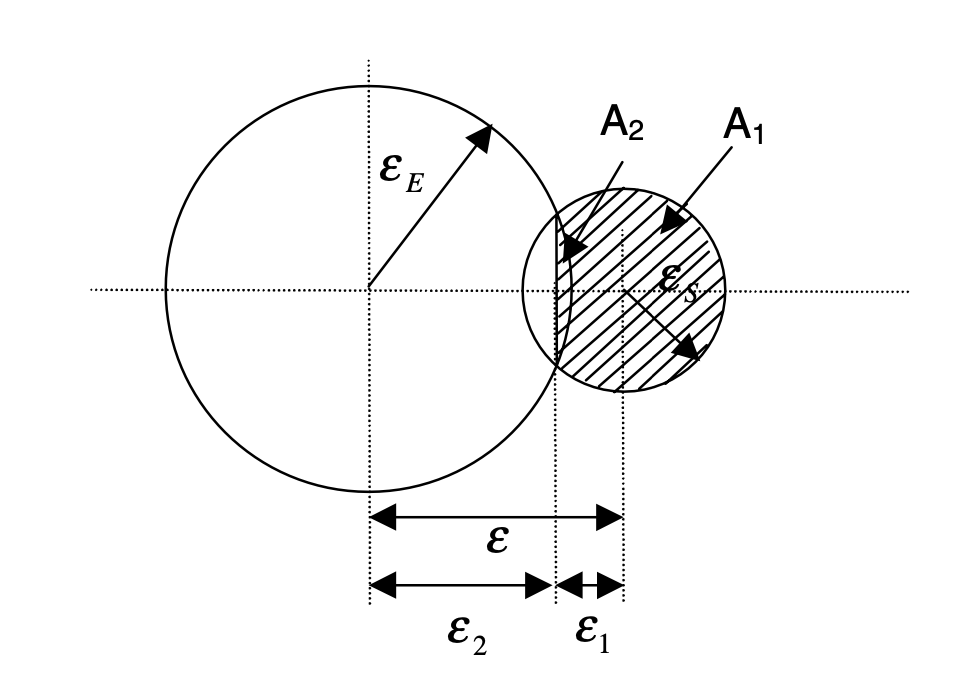
\includegraphics[width=\figmed]{angle_defs_krag_520.png}
  \caption{Angle and area definitions for penumbra shadowing, Figure 5.20 in \cite{krag2003}}
  \label{fig:penumbra_angles}
\end{figure}
\graphicspath{{/Users/liamrobinson/Documents/msthesis/static_images/aas_2022_figs}}

In Eq \ref{eq:irradiance_fraction_angles}, $\epsilon_s$ is the half-angle of the Sun disk at the object, $\epsilon_e$ is the half-angle of the Earth disk from the object as a function of the geodetic latitude of the object $\phi_{obj}$. Additionally, $\epsilon$ is the angle between the center of the Earth and Sun from the perspective of the object, with $\epsilon_1$ and $\epsilon_2$ being the angles from the center of the Sun and Earth disks to the center of their overlap, if it exists \cite{krag2003}. These angles are defined in Figure \ref{fig:penumbra_angles}. Given these angles, the illumination fraction $f_{Sun}$ is computed:

\begin{equation} \label{eq:irradiance_fraction}
  f_{Sun} = \begin{cases}
    1 & \epsilon \geq (\epsilon_s + \epsilon_e) \\ 
    0 & \epsilon \leq (\epsilon_e - \epsilon_s) \\ 
    \frac{a_1 - a_2}{\pi \epsilon_s^2} & \mathrm{else}
  \end{cases}.
\end{equation}

In Eq \ref{eq:irradiance_fraction}, the solid angles $a_1$ and $a_2$ are defined in Figure \ref{fig:penumbra_angles} and are computed via:

\begin{align*} \numberthis \label{eq:penumbra_areas}
  a_1 &= \pi \epsilon_s^2 - \epsilon_s^2 \cos^{-1} \left(\frac{\epsilon_1}{\epsilon_s}\right)
    + \epsilon_1 \sqrt{\epsilon_s^2 - \epsilon_1^2} \\
  a_2 &= \epsilon_e^2 \cos^{-1}\left(\frac{\epsilon_2}{\epsilon_e} \right) - \epsilon_2 \sqrt{\epsilon_e^2 - \epsilon_2^2} \\
\end{align*}

Computing Eq \ref{eq:irradiance_fraction} for a dense grid of points in the J2000 reference frame reveals the geometry of the penumbra and umbra in Figure \ref{fig:penumbra}, illustrating that the penumbra expands into the umbra as the observer recedes from the Earth. 

\graphicspath{{/Users/liamrobinson/Documents/PyLightCurves/docs/build/html/_images}}
\begin{figure}[!htb]
  \centering
  \includegraphics[width=\figbig]{sphx_glr_penumbra_plane_001.png}
  \caption{Shadow fraction in J2000, effect exaggerated by scaling the Sun radius by a factor $10$}
  \label{fig:penumbra}
\end{figure}
\graphicspath{{/Users/liamrobinson/Documents/msthesis/static_images/aas_2022_figs}}

\subsubsection{SNR}

As the signal-to-noise ratio of an object signal on the CCD pixel grid degrades, it becomes more difficult to determine whether an object is present at all. Given a minimum limiting SNR $\mathrm{SNR}_{min}$ this constraint takes the form:

\begin{equation} \label{eq:moon_exclusion}
  \nu_{\mathrm{SNR}} = \begin{cases}
    1 & \mathrm{SNR} > \mathrm{SNR}_{min}\\
    0 & \mathrm{else}
  \end{cases}.
\end{equation}

In Eq \ref{eq:moon_exclusion}, $\nu_{\mathrm{SNR}} = 1$ implies that the observation is valid, with $\nu_{\mathrm{SNR}} = 0$ implying that the object signal cannot be discerned from the image background.

\subsubsection{Moon Exclusion Angle}

Focusing the irradiance of the Moon onto the sensor grid will seriously damage the CCD. For the Purdue Optical Ground Station, straylight from the Moon begins leaking into the optics around $30^\circ$ from the center of the Moon disk. This observation constraint is imposed for an arbitrary exclusion angle $\theta_{Moon,ex}$ via:

\begin{equation} \label{eq:moon_exclusion}
  \nu_{Moon} = \begin{cases}
    1 & \cos^{-1}\left( \frac{\left( \vctr{r}_{Moon} - \vctr{r}_{obs} \right) \cdot \left( \vctr{r}_{obj} - \vctr{r}_{obs} \right)}{\| \vctr{r}_{Moon} - \vctr{r}_{obs} \| \| \vctr{r}_{obj} - \vctr{r}_{obs} \|} \right) > \theta_{Moon,ex}\\
    0 & \mathrm{else}
  \end{cases}.
\end{equation}

In Eq \ref{eq:moon_exclusion}, $\nu_{Moon} = 1$ implies that the observation is valid, with $\nu_{Moon} = 0$ implying that the observation is too close to the Moon.

\subsubsection{Minimum Elevation}

Due to the local topology at the observer location, an operator may assign a minimum angle from the horizon $\theta_{elev,min}$ for observations. Approximating the station inertial position $\vctr{r}_{obs}$ as being aligned with zenith, this yields the condition:


\begin{equation} \label{eq:elevation_exclusion}
  \nu_{elevation} = \begin{cases}
    1 & 90^\circ - \cos^{-1}\left( \frac{\left( \vctr{r}_{obj} - \vctr{r}_{obs} \right) \cdot \left( \vctr{r}_{obs} \right)}{\| \vctr{r}_{Moon} - \vctr{r}_{obs} \| \| \vctr{r}_{obs} \|} \right) > \theta_{Moon,ex}\\
    0 & \mathrm{else}
  \end{cases}.
\end{equation}

In Eq \ref{eq:moon_exclusion}, $\nu_{elevation} = 1$ implies that the observation is valid, with $\nu_{elevation} = 0$ implying that the observation is too close to the horizon.

\subsection{Mean Irradiance at The Observer}

Given the normalized irradiance computed via Eq \ref{eq:lc_func_normalized} for convex objects or Eq \ref{eq:lc_normalized_engine} for any object shaded using Algorithm \ref{alg:pix_shading}, the recieved mean irradiance at the telescope aperture is given by:

\begin{equation} \label{eq:mean_irrad_at_aperture}
  \bar{I} = \nu_{Moon,ex} \cdot \nu_{elevation} \cdot \nu_{\mathrm{SNR}} \frac{I_0 f_{Sun} \hat{I}}{\left( \vctr{r}_{obj} - \vctr{r}_{obs} \right)^2}.
\end{equation}

In order to sample a noisy light curve, this mean irradiance must be converted into a mean photoelectron count via Eq \ref{eq:sint}, yielding $\bar{C}_{all}$.

\subsection{Sampling Noisy Light Curves} \label{sec:sampling_lcs}

Given the irradiance of the object observed by the telescope, the noisy light curve is computed by building a grid containing the object signal, background noise, and sensor noise. On a pixel-by-pixel basis, the mean object signal is given by an alteration of Eq \ref{eq:airy_gaussian}:

\begin{equation} \label{eq:obj_signal_grid}
  \bar{C}_{obj}(x, y) = \frac{0.838 \bar{C}_{all}}{2 \pi \sigma^2} \exp\left( - \frac{(x - x_0)^2 + (y - y_0)^2}{2 \sigma^2  s_{pix}^2} \right).
\end{equation}

In Eq \ref{eq:obj_signal_grid}, $\left(x_0, y_0\right)$ are the exact pixel coordinates of the object centroid, $\sigma$ is the Gaussian standard deviation from Eq \ref{eq:airy_variance} in arcseconds, and $s_{pix}$ is the pixel scale in arcseconds per pixel. Likewise, the total noise sampled in each pixel is given by samples from all the relevant source distributions:

\begin{equation} \label{eq:noise_signal_grid}
  C_{noise} = N_{background} + N_{dark} + N_{trunc} + N_{read}.
\end{equation}

In Eq \ref{eq:noise_signal_grid}, $N_{background}$ is a sample drawn from $\mathrm{Pois}(\lambda_{background})$, $N_{dark}$ is drawn from $\mathrm{Pois}(\Delta t \cdot \lambda_{dark})$, $N_{trunc}$ is drawn from $\mathrm{Uniform}(-g/2, g/2)$, and $N_{read}$ is drawn from $\mathrm{Normal}(0, \sigma_{read}^2)$. 

Assuming perfect knowledge of the image background mean in the region around the object signal --- a reasonable assumption given that there are generally millions of background pixels in the image --- the counts $C_{obj,meas}$ attributed to the object pixels $\{x_{obj}, y_{obj}\}$ is given by:

\begin{align*} \numberthis \label{eq:noisy_counts}
  C_{noise,all} &= \sum_{i=1}^{A_{airy}}{C_{noise,i}} \\
  C_{obj,all} &= \sum_{x \in x_{obj}, \: y \in x_{obj}}{\bar{C}_{obj}(x, y)} \\
  C_{obj,meas} &= C_{noise,all} - A_{airy} \left( \Delta t \cdot \lambda_{dark} + \lambda_{background} \right) 
\end{align*}

In Eq \ref{eq:noisy_counts}, $A_{airy}$ is the area of the central maximum of the Airy disk in square pixels presented in Eq \ref{eq:airy_area}. The measured object signal $C_{obj,meas}$ can then be transformed into irradiance via Eq \ref{eq:count_to_irrad}:

\begin{equation}
  I_{obj,meas} = \frac{C_{obj,meas}}{\mathrm{SINT} \cdot \Delta t}
\end{equation}

or to apparent magnitude by applying Eq \ref{eq:mag_to_irradiance}:

\begin{equation}
  m_{obj,meas} = -2.5 \log_{10}\left( \frac{I_{obj,meas}}{I_z} \right)
\end{equation}

or normalized irradiance by applying Eq \ref{eq:irradiance_to_norm_irradiance}:

\begin{equation}
  \hat{I}_{obj,meas} = \frac{\| \vctr{r}_{obj} - \vctr{r}_{obs} \|^2}{I_0} I_{obj,meas}.
\end{equation}